\section{State}

O padrão \textit{State} permite alterar o comportamento de um objeto 
alterando seu estado interno. As operações que dependem do 
estado do objeto são definidas em uma interface conhecida 
pelo objeto, de forma que ele delegue essas operações 
para outra classe que implemente essa interface.\cite{gamma:1995} 

Essa abordagem contribui para o reuso de operações 
que se repetem em classes relacionadas. Sem o \textit{State}, 
essas classes teriam que ser instanciadas novamente 
a cada mudança de estado. Outra vantagem é que o 
padrão permite que o estado seja trocado dinamicamente 
durante a execução. A estrutura do padrão pode ser 
vista na Figura \ref{state_struct}.

\begin{figure}[htb]
	\caption{\label{state_struct}Estrutura do \textit{State}.}
	\begin{center}
	    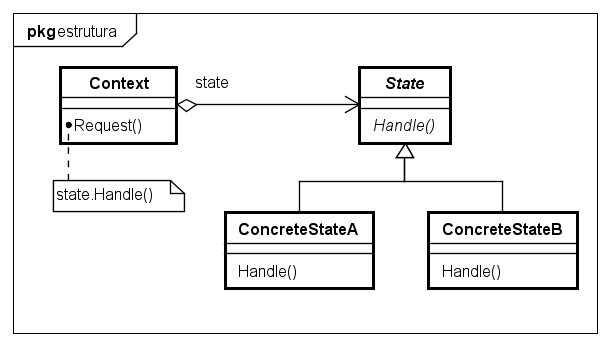
\includegraphics[scale=0.5]{5_padroes-contexto-funcional/5.3_comportamentais/5.3.08_state/state_estrutura.png}
	\end{center}
  \caption*{Fonte: O Autor (2021)}
\end{figure}

\subsection*{Exemplo Orientado a Objetos}

Como exemplo, é considerada uma classe \texttt{TCPConnection} 
que define uma conexão de rede que pode estar em diversos 
estados: Estabelecida, Escutando e Fechada. Dependendo 
do estado em que a conexão se encontra, ela deve 
responder de forma diferente às operações que uma 
conexão TCP pode realizar. O padrão \textit{State}, cuja 
implementação pode ser vista no diagrama da Figura 
\ref{state_exemplo} e no Código \ref{oostate}, é 
utilizado para encapsular em classes diferentes as 
operações referentes a cada estado da conexão. 
Dessa forma, a classe \texttt{TCPConnection} delega a uma classe 
que implementa a interface \texttt{TCPState} a execução das 
operações necessárias. Quando o estado interno da classe 
for modificado, a operação referente ao novo estado 
também será alterada automaticamente.

\begin{figure}[htb]
	\caption{\label{state_exemplo}Exemplo de \textit{State}.}
	\begin{center}
	    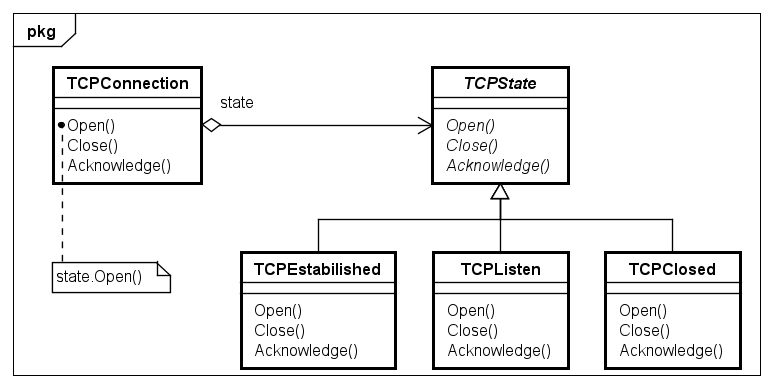
\includegraphics[scale=0.5]{5_padroes-contexto-funcional/5.3_comportamentais/5.3.08_state/state_exemplo.png}
	\end{center}
  \caption*{Fonte: O Autor (2021)}
\end{figure}

\begin{lstlisting}[caption={\textit{State} Orientação a Objetos.},label=oostate]

class TCPConnection(var state : TCPState) {
  def Open(): Unit = state.Open()
  def Close(): Unit = state.Close()
  def Acknowledge(): Unit = state.Acknowledge()
}

trait TCPState {
  def Open()
  def Close()
  def Acknowledge()
}

class TCPEstabilished extends TCPState {
  def Open():Unit = {
    //Implementação para conexão estabelecida
  }
  def Close(): Unit = {
    //Implementação para conexão estabelecida
  }
  def Acknowledge(): Unit = {
    //Implementação para conexão estabelecida
  }
}

class TCPListen extends TCPState {
  def Open():Unit = {
    //Implementação para conexão escutando
  }
  def Close(): Unit = {
    //Implementação para conexão escutando
  }
  def Acknowledge(): Unit = {
    //Implementação para conexão escutando
  }
}

class TCPClosed extends TCPState {
  def Open():Unit = {
    //Implementação para conexão fechada
  }
  def Close(): Unit = {
    //Implementação para conexão fechada
  }
  def Acknowledge(): Unit = {
    //Implementação para conexão fechada
  }
}

\end{lstlisting}
\legend{Fonte: O Autor (2021)}

\subsection*{Contexto Funcional}

Para que o comportamento de um valor possa 
ser alterado ao alterar seu estado, ele 
pode ser encapsulado dentro de outro valor. 
No Código \ref{fpstate}, o tipo \texttt{TCPState} 
é declarado na linha 2, onde armazena 
três funções: uma para a ação \textit{open}, 
uma para a ação \textit{close} e uma para 
a ação \textit{acknowledge}. Da mesma forma, 
as operações \texttt{Open}, \texttt{Close} e \texttt{Acknowledge}, 
definidas em seguida, recebem como 
parâmetro uma tupla do tipo \texttt{TCPState} e 
executam as funções desejadas.

\begin{lstlisting}[caption={\textit{State} Funcional.},label=fpstate]
    
type TCPState = (() => Unit,
                 () => Unit,
                 () => Unit)

def Open(state : TCPState) : Unit = state._1()

def Close(state : TCPState) : Unit = state._2()

def Acknowledge(state : TCPState) : Unit = state._3()
    
\end{lstlisting}
\legend{Fonte: O Autor (2021)}

O Código \ref{fpstate2} demonstra como seriam 
declaradas as tuplas para cada estado visto 
no exemplo orientado a objetos. Dessa forma, 
os valores \texttt{TCPEstabilished}, \texttt{TCPClosed} e 
\texttt{TCPListen} são utilizados para definir que 
tipo de comportamento o programa deverá 
adotar para cada estado possível.

\begin{lstlisting}[caption={\textit{State} Funcional.},label=fpstate2]
    
val TCPEstabilished = (
  () => {
    //Operação Open para conexão estabelecida
  },
  () => {
    //Operação Close para conexão estabelecida
  },
  () => {
    //Operação Acknowledge para conexão estabelecida
  }
)

val TCPClosed = (
  () => {
    //Operação Open para conexão fechada
  },
  () => {
    //Operação Close para conexão fechada
  },
  () => {
    //Operação Acknowledge para conexão fechada
  }
)

val TCPListen = (
  () => {
    //Operação Open para conexão escutando
  },
  () => {
    //Operação Close para conexão escutando
  },
  () => {
    //Operação Acknowledge para conexão escutando
  }
)
    
\end{lstlisting}
\legend{Fonte: O Autor (2021)}